\documentclass[../main.tex]{subfiles}

\begin{document}

	\section{Features}

	As stated previously, the problem formulation into a classification problem implies that features should be extracted from the input data along with the DSM and Orthoimage. The extracted features will be fed to classifiers in order to train and further predict errors.\\

	\subsection{Raw features}


	The first step was to extract low level features and expose them so that we can engineer sophisticated ones to train the classifiers on. In fact, for each building,the facet adjacency graph is computed --- \textit{c.f.} Figure~\ref{fig::geom_features} --- with meaningful information for each facet. We also computed the buildings orthoprojection\footnote{Projection on the Plane $(O, \vec{\imath}, \vec{\jmath})$} and stored it in vector --- \textit{c.f.} Figure~\ref{fig::vector} --- and raster mode --- \textit{c.f.} Figure~\ref{fig::raster}.\\

	\thisfloatsetup{heightadjust=object}
	\begin{figure}[H]
		\ffigbox[\FBwidth]
		{
			\begin{subfloatrow}[2]
				\captionsetup{labelformat=brace, justification=raggedright}
				\ffigbox[\FBwidth]
				{\caption{Raster orthoprojection.}\label{fig::raster}}{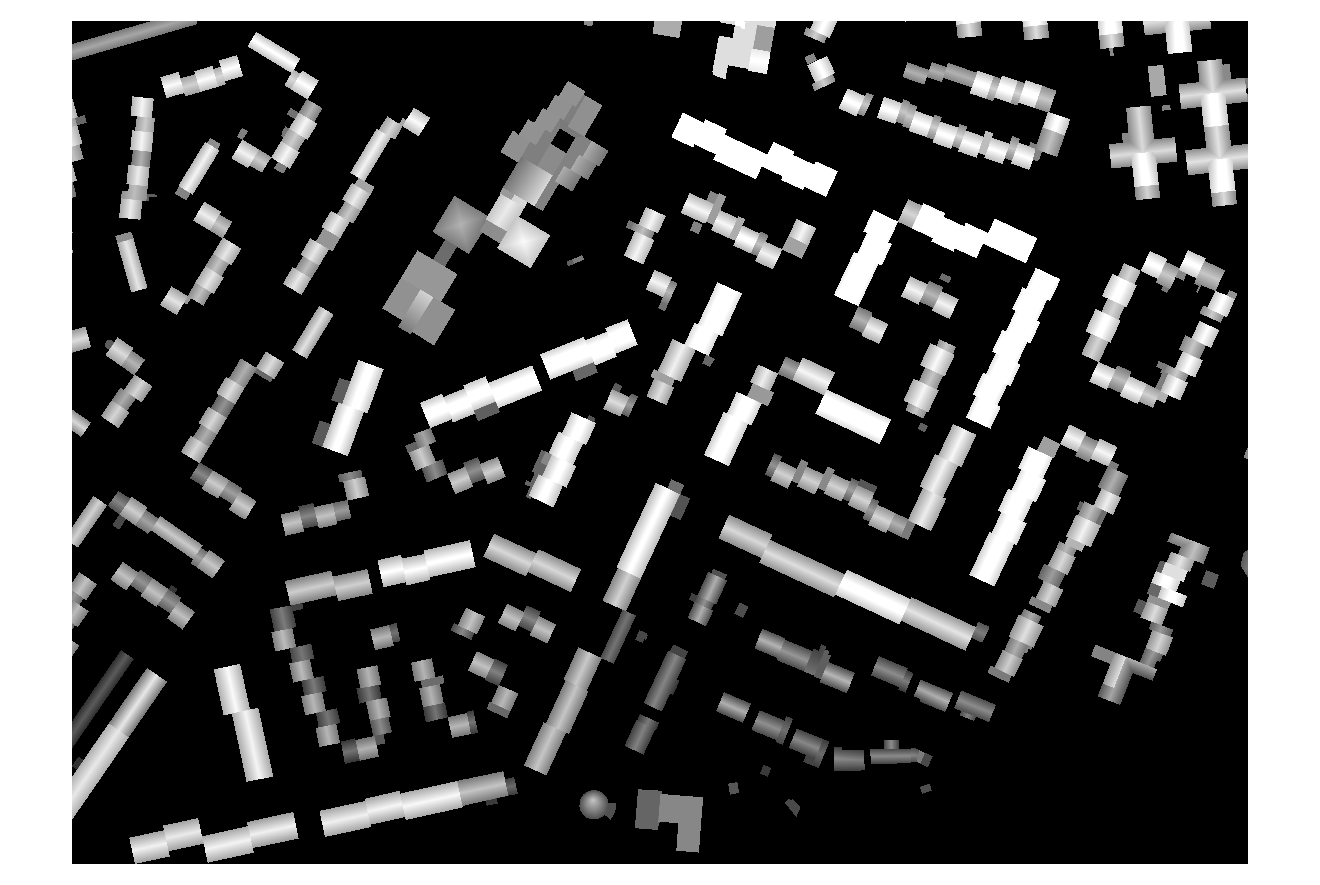
\includegraphics[width=.48\textwidth]{../images/raster/raster_projection}}
				\ffigbox[\FBwidth]{\caption{Vector orthoprojections (in transparent blue).}\label{fig::vector}}{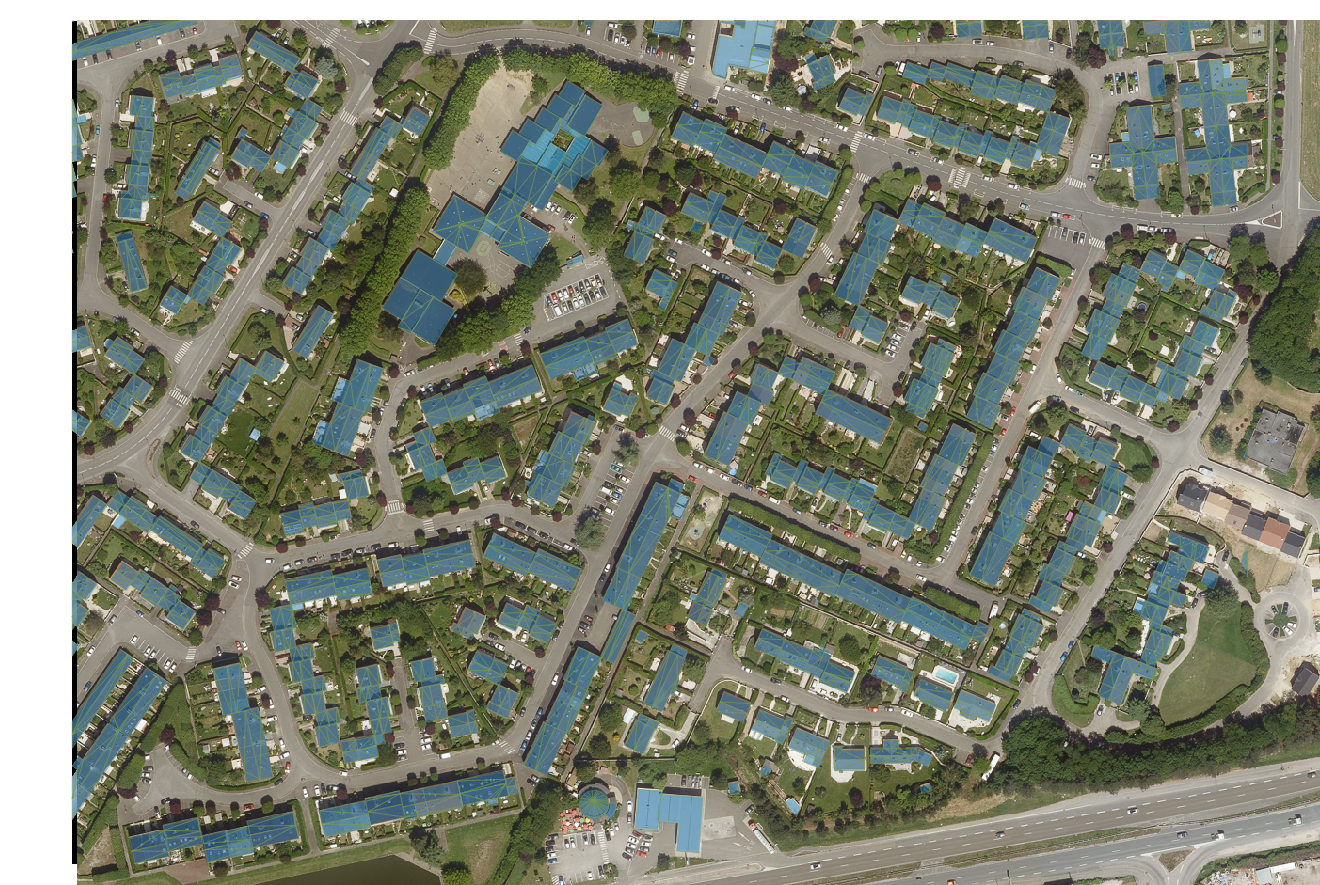
\includegraphics[width=.48\textwidth]{../images/raster/vector_projection}}
			\end{subfloatrow}
		}
		{
			\caption{\label{fig::orthoproj}Scene orthoprojections.}
		}
	\end{figure}

	\begin{figure}[H]
		\includestandalone[mode=buildnew, scale=1]{dual_features}
		\caption{\label{fig::geom_features} Low level geometric features per building.}
	\end{figure}
	\clearpage

	\subsection{Mid level features}
~\\

	The previous features are raw and not useful for classification. As a first
	step, in order to establish a baseline for the qualification, simple
	features were chosen. They could be subdivided as follows:
	\begin{itemize}
		\item[(i).] Geometric --- or intrinsic --- features: based on the graph adjacency features and the vector orthoprojections, I tried the feature vector per building in equation~\ref{eq::feature_vec}:
		\begin{equation}\label{eq::feature_vec}
			\text{feature\_vector} = \begin{bmatrix}
				statistics(degree_{facets})\\
				statistics(areas_{facets})\\
				statistics({facets\_centroid\_distances}_{facets})\\
				statistics({angles\_btw\_normals}_{facets})\\
				statistics(nomals\_with\_relations_{facets})\\
				statistics(areas_{projected\_facets})\\
				statistics(length_{projected\_edges})
		\end{bmatrix}
		\end{equation}
		where:
		\begin{equation}
			statistics: property \mapsto \begin{bmatrix}
			\max_{facets}(property)\\
			\min_{facets}(property)\\
			mean_{facets}(property)\\
			median_{facets}(property)
		\end{bmatrix}
		\end{equation}
		or:
		\begin{equation}
			statstics: property \mapsto histogram(property, *args)
		\end{equation}
		\item[(ii).] Altimetric features: using the raster projections and the provided DSM, I computed the difference and used the its histogram or statistics --- like before --- as a feature vector.
		\item[(iii.)] Image features: left for later.
	\end{itemize}

	For now, we have focused on geometric features and altimetic features to complete the whole classification pipeline.The graph kernel methods and ortho image features are left for later. I should also grow my labelled datasets and invistigate other regions by active learning: transforming the pipeline to an active setting.

	The features are extracted building wide. However, we can try to extract features per facets and thus qualify facet instances not the whole building. We can thus localize the erronous facets. This approach can be coupled to the first one or compared against.
\end{document}
